\section{Aplikacja dla komputerów stacjonarnych}
\label{sec:java-app}
Na potrzeby prezentacji biblioteki zarządzającej robotem Dark Explorer napisanej
w języku Java, stworzono aplikację dla komputerów stacjonarnych. Można ją
uruchomić na wielu systemach operacyjnych, między innymi na systemach Windows
oraz Linux. Aplikacja demonstracyjna korzysta z przygotowanej na rzecz tej pracy
magisterskiej biblioteki zarządzającej robotem oraz z biblioteki wspierającej JSR
82. Z pośród wielu bibliotek przedstawionych w tabeli \ref{tab:JSR82SDK} wybrana
została bibloteka BlueCove\cite{website:bluecove.org}. Działa ona pod wieloma
systemami operacyjnymi, jest darmowa dla zastosowaniach niekomercyjnych oraz
posiada dokumentację wraz z przykładowymi aplikacjami.

Przygotowany program zarządzający robotem pozwala na zaprezentowanie wszystkich
jego funkcjonalności stworzonych podczas rozwoju tej pracy magisterskiej. Rysunek
\ref{fig:java-desk-app} przedstawia ekran główny wspomnianej aplikacji. Funkcjonalności tej aplikacji są identyczne z tymi opisanymi w rozdziale \ref{subsec:sdk-.net}.

\begin{figure}[!ht]
 \centering
 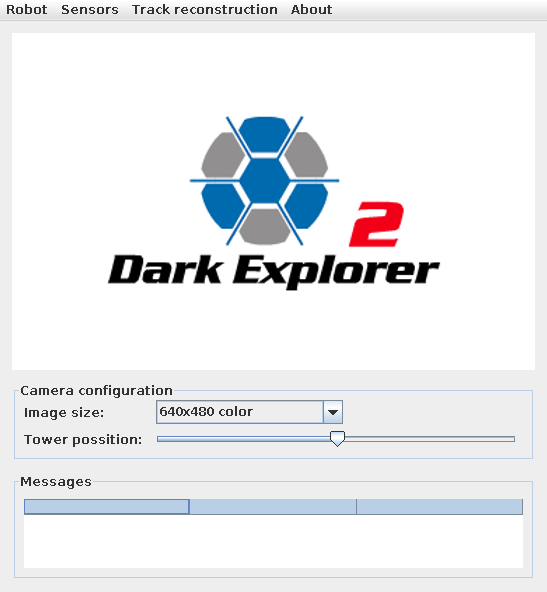
\includegraphics[height=130mm]{../images/ch03/java-desk-app.png}
 \caption{Okno główne aplikacji sterującej napisanej w języku Java}
 \label{fig:java-desk-app}
\end{figure}